% #############################################
	\section{Methods} \label{sec:system}
% #############################################


The proposed system consists of several stages, namely: time series segmentation and feature extraction from  FHR signals; similarity calculation with NCD, for which the combination of similarity matrices can provide with further advantage; and choice of a suitable classification algorithm for the final purpose of hypoxia detection. The theoretical basis and design criteria of these stages are described below.



%#############################################################################################
\subsection{Permutation Entropy}
%#############################################################################################

Here your code



%%##########################################################
\subsection{Time Irreversibility}
%##########################################################
Here your code


%%##########################################################
\subsection{Test Hypothesis Bootstrap}
%%##########################################################
Here your code



%##########################################################
% Section data description
%##########################################################
\section{Data description}\label{sec:data}
\myblue{FHR  records\footnote{Data  is available from the website: http://sites.google.com/site/hufahypoxia.} were acquired with a Philips cardiotocograph for a total of 32 recordings, 15 controls and 17 cases. A case was declared whether: 1) the PH of the umbilical artery was $\leq$ 7.05; or 2) the APGAR score was $\leq$ 7 at 5 minutes after delivery  and a reanimation type III or greater was required. The institutional Medical Ethics Review Board approved the use of this data.}

\myblue{Records, see Figure~\ref{fig:RAWFHR} for an example, have considerable variability both in start/ending times and  pauses as labor duration vary. In addition, the cardiotocograph may be disconnected at any time for a number of reasons. Also, the signal is lost sometimes as the fetus and mother move.  The  cardiotocograph provides three signal qualities (lost, medium and high). We decided to consider the window between 4 to 1 hours before birth for our analysis, even though not all patients have signal along all this window, e.g. nine patients even start being monitored after 4 hours to delivery (8 cases) or they are removed the cardiotocograph before  1 hour to delivery (one case). When a patient has no signal in the entire interval analyzed in a experiment, it was excluded (see below).}

%\textcolor{declared-color}{text}
\begin{figure}[tp]
\centering%
\subfigure[hypoxic]{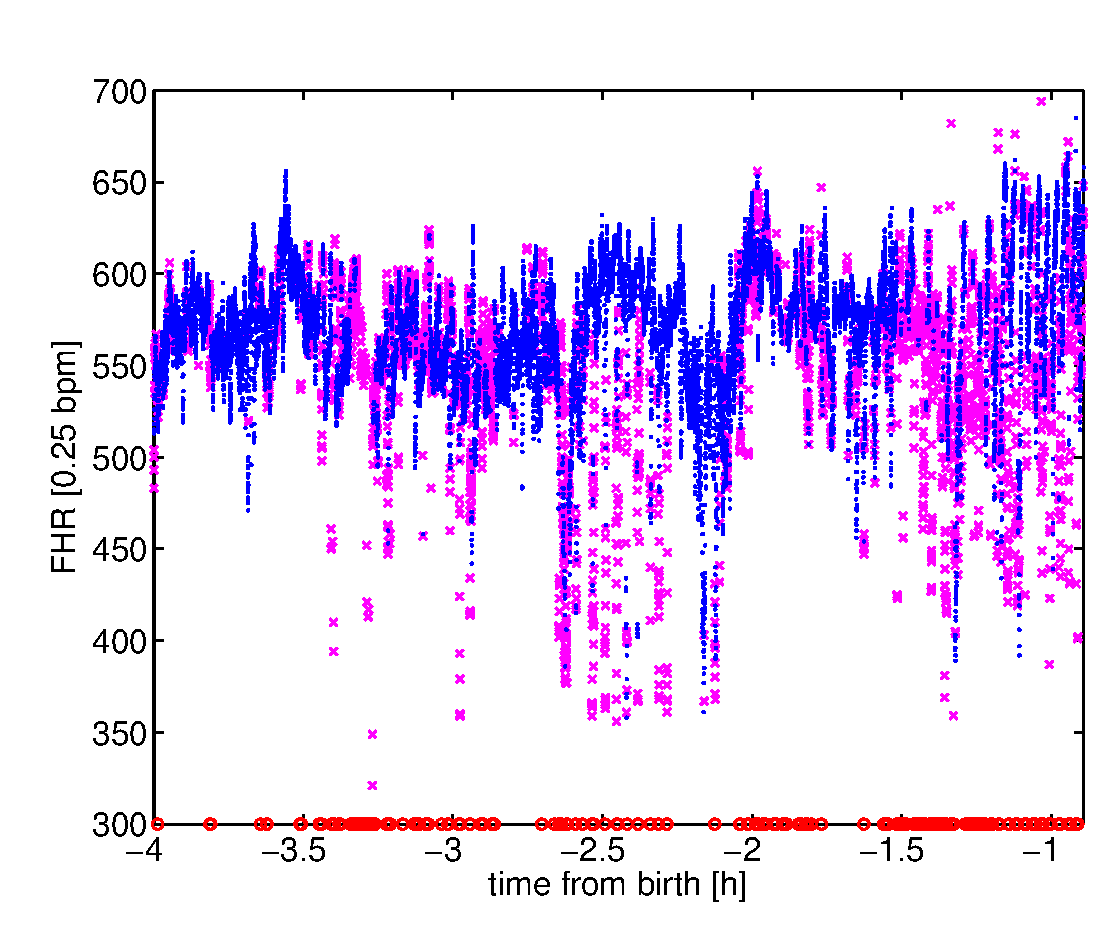
\includegraphics[width=0.9\linewidth]{./figs/caso}}\\%
\subfigure[control]{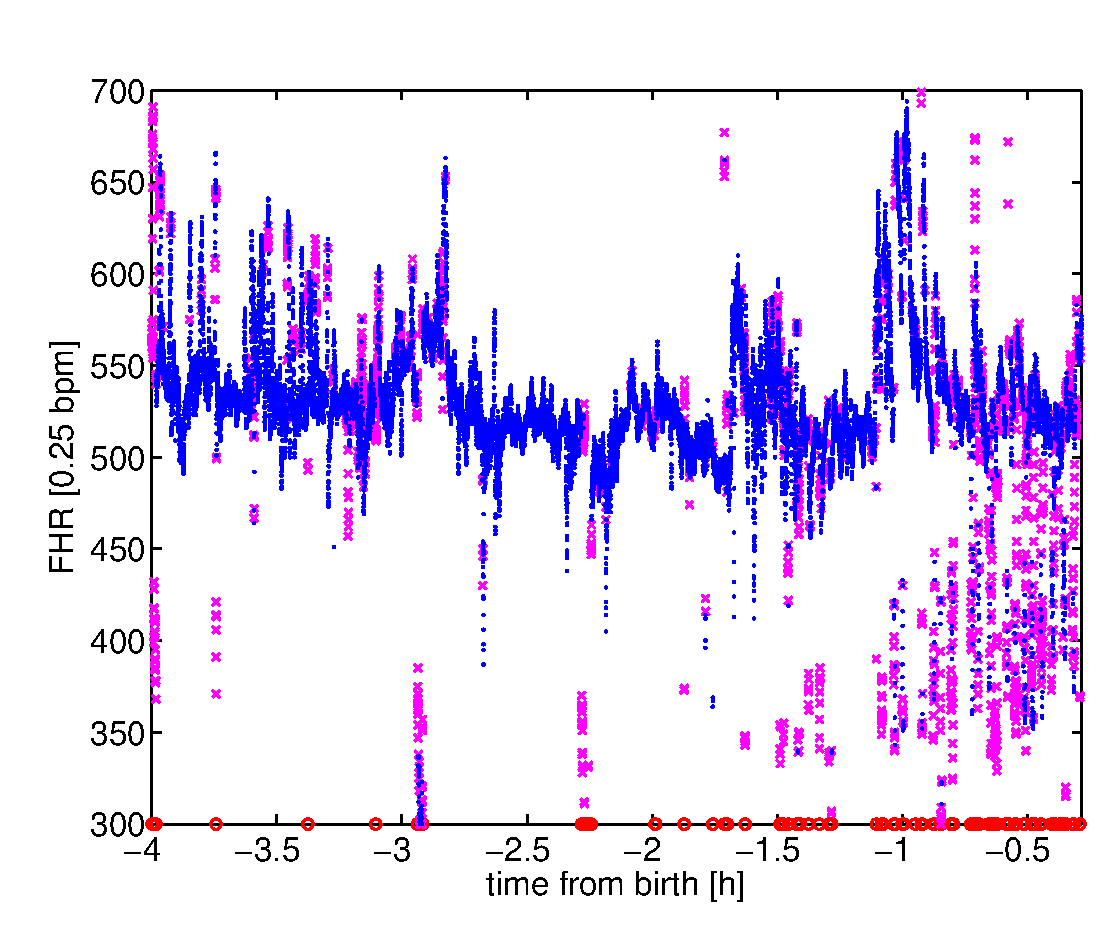
\includegraphics[width=0.9\linewidth]{./figs/control}}
\caption{FHR for (a) a hypoxic and (b) a control patient. Signal qualities are 9.9\% lost, 19.2\% medium and 70.9\% high for (a) ; and 1.8\% lost, 9.8\% medium and 88.3\% high for (b).  Signal qualities  high, medium and lost  are respectively represented by the markers: ``\textcolor{blue}{$\cdot$}'', ``\textcolor{magenta}{x}'' and ``\textcolor{red}{o}''.}
\label{fig:RAWFHR}
\end{figure}
%##########################################################
% Section data description
%##########################################################


